\section{Módulo de Registro}

	O Módulo de Registro é responsável por cadastrar novos usuários no sistema e treiná-lo para também reconhecer esse novo usuário. Basicamente, o processo de registro, ilustrado na Figura~\ref{fig:registro}, segue as seguintes etapas :

		\begin{figure}[H]
			\begin{center}
				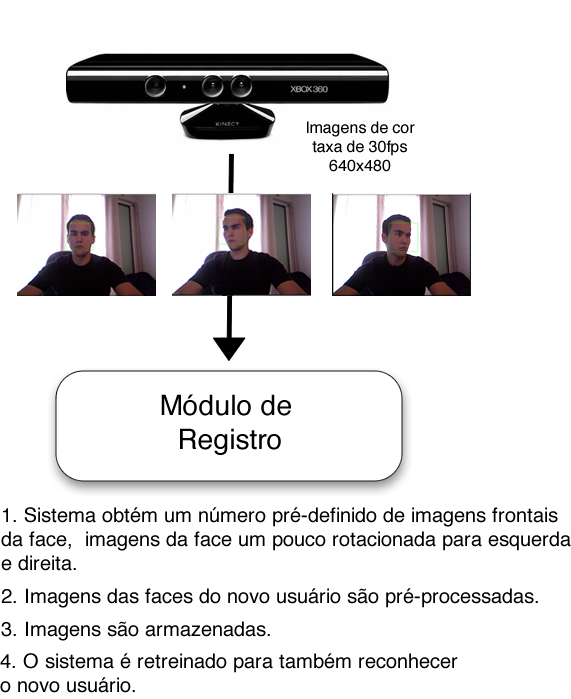
\includegraphics[scale=1.5]{figuras/4.ProblemaEProposta/registro.png}
			\end{center}
			\caption{Módulo de Registro do Sistema TRUE.}
			\label{fig:registro}
		\end{figure}		

		\begin{enumerate}
			\item O novo usuário fica em uma posição fixa e frontal em relação ao \textit{Kinect}. 
			\item O sistema obtém seis imagens frontais do usuário.
			\item O usuário, então, deve rotacionar um pouco a face para a esquerda e o sistema obtém mais duas imagens do usuário. Depois, deve rotacionar um pouco para direita e o sistema obtém outras duas imagens do usuário.
			\item As imagens obtidas são processadas: as imagens são convertidas em escala de cinza, novas imagens são criadas recortando a região da face encontrada, as imagens, então, são redimensionadas e equalizadas criando assim uma padrão de tamanho, brilho e contraste nas imagens.
			\item Armazena-se as imagens.
			\item O sistema é treinado para, também, reconhecer esse usuário.
		\end{enumerate}

	Após o treinamento, o Sistema TRUE reiniciará para que o reconhecimento seja feito utilizando as novas informações obtidas com o treinamento.

	Como descrito, durante o processo de captura das imagens, o usuário deve rotacionar a face um pouco para direita e para esquerda obtendo, além de imagens frontais, imagens um pouco mais de perfil do usuário, como mostrado na Figura~\ref{fig:imgs-cadastro}. Isso foi feito para que o sistema se torne um pouco mais robusto em relação a posição da face dos usuários ao tentar reconhece-los.

		\begin{figure}[H]
			\begin{center}
				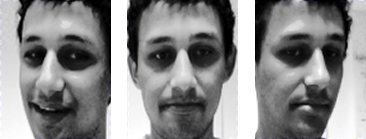
\includegraphics[scale=0.4]{figuras/4.ProblemaEProposta/face-registro.png}
			\end{center}
			\caption{Exemplo de imagens resultantes do cadastro do usuário.}
			\label{fig:imgs-cadastro}
		\end{figure}	

	A última etapa do módulo de registro consiste no treinamento do sistema, descrito na Figura~\ref{fig:treinamento}.

		\begin{figure}[hbt]
			\begin{center}
				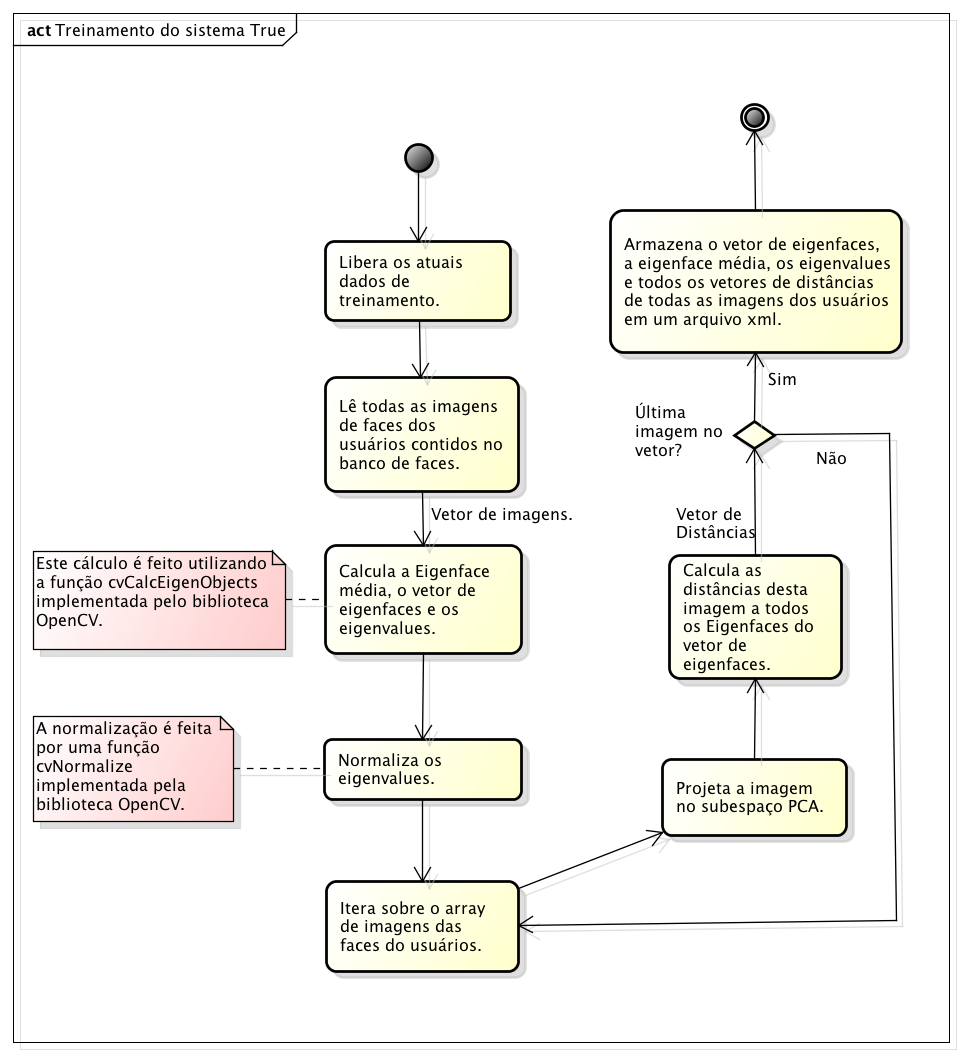
\includegraphics[scale=0.7]{figuras/4.ProblemaEProposta/diagrama-registro.png}
			\end{center}
			\caption{Fluxo básico do treinamento do Sistema TRUE.}
			\label{fig:treinamento}
		\end{figure}	